\section{Content of enclosed CD}
\label{appendix:cd-contents}


    \begin{enumerate}
    \item $/docs/$ - Documentation of the PDSurvey platform
    \item $/pdsurvey/$ - Source Code for the PDSurvey platform
    \item $/pdemail/$ - Python Script for sending Emails from the Balloon Shooter Game
    \item $/pdclient-static/$ - A copy of PDClient, the interface users saw
    \item Google Docs - 
    \item $/interviews/$ - The audio recordings of all interviews conducted during the field study, including a transcribed version
    \item $/thesis/$ - LaTeX version of the thesis
    \item \textbf{TODO} noch einige Ordner mehr...
    \end{enumerate}



%% - - -  D O C U M E N T A T I O N  - - - %%
\section{Documentation of PDSurvey Platform}
\label{appendix:documentation}

  A user, developer and maintenance documentation for the PDSurvey platform can be found in the GitHub repository: \url{https://github.com/lukasziegler/masterarbeit/tree/master/docs} and on the enclosed CD $/docs/$.



%% - - - -  P A P E R S   R E A D  - - - - %%
\clearpage
\section{Papers Evaluating Public Displays}
  
  List of relevant papers, which include an evaluation of public displays.

  TABLE: 1st column (paper), 2nd column evaluation (quantitative, qualitative, no evaluation)

  TODO



%% - - - I N T E R V I E W S   C A R R I E D   O U T  - - - %%
\clearpage
\section{Questionnaires for Field Study}
\label{appendix:interviews}

  \label{appendix:interview-participant}
  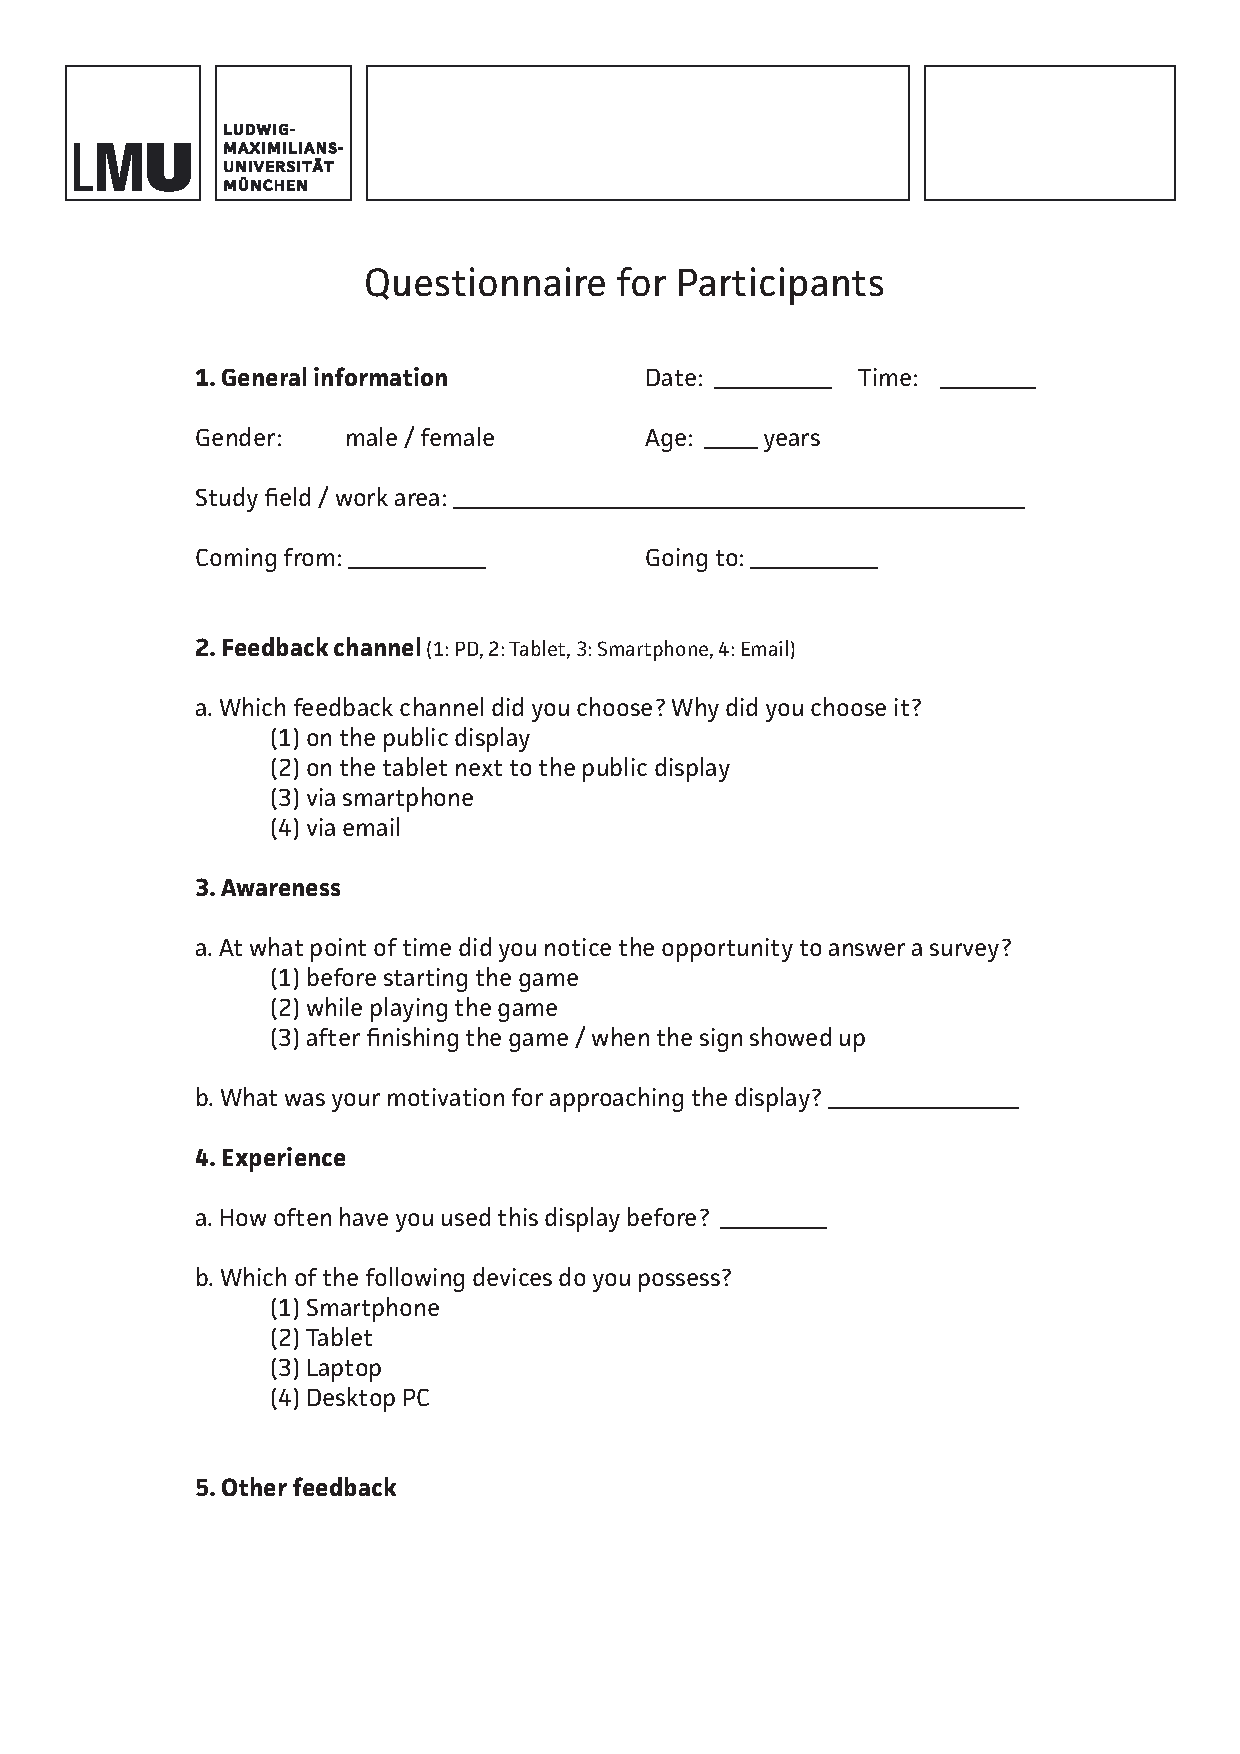
\includepdf[pages={-},scale=.9,pagecommand={}]{pdf/interview-participants.pdf}

  \label{appendix:interview-passerby}
  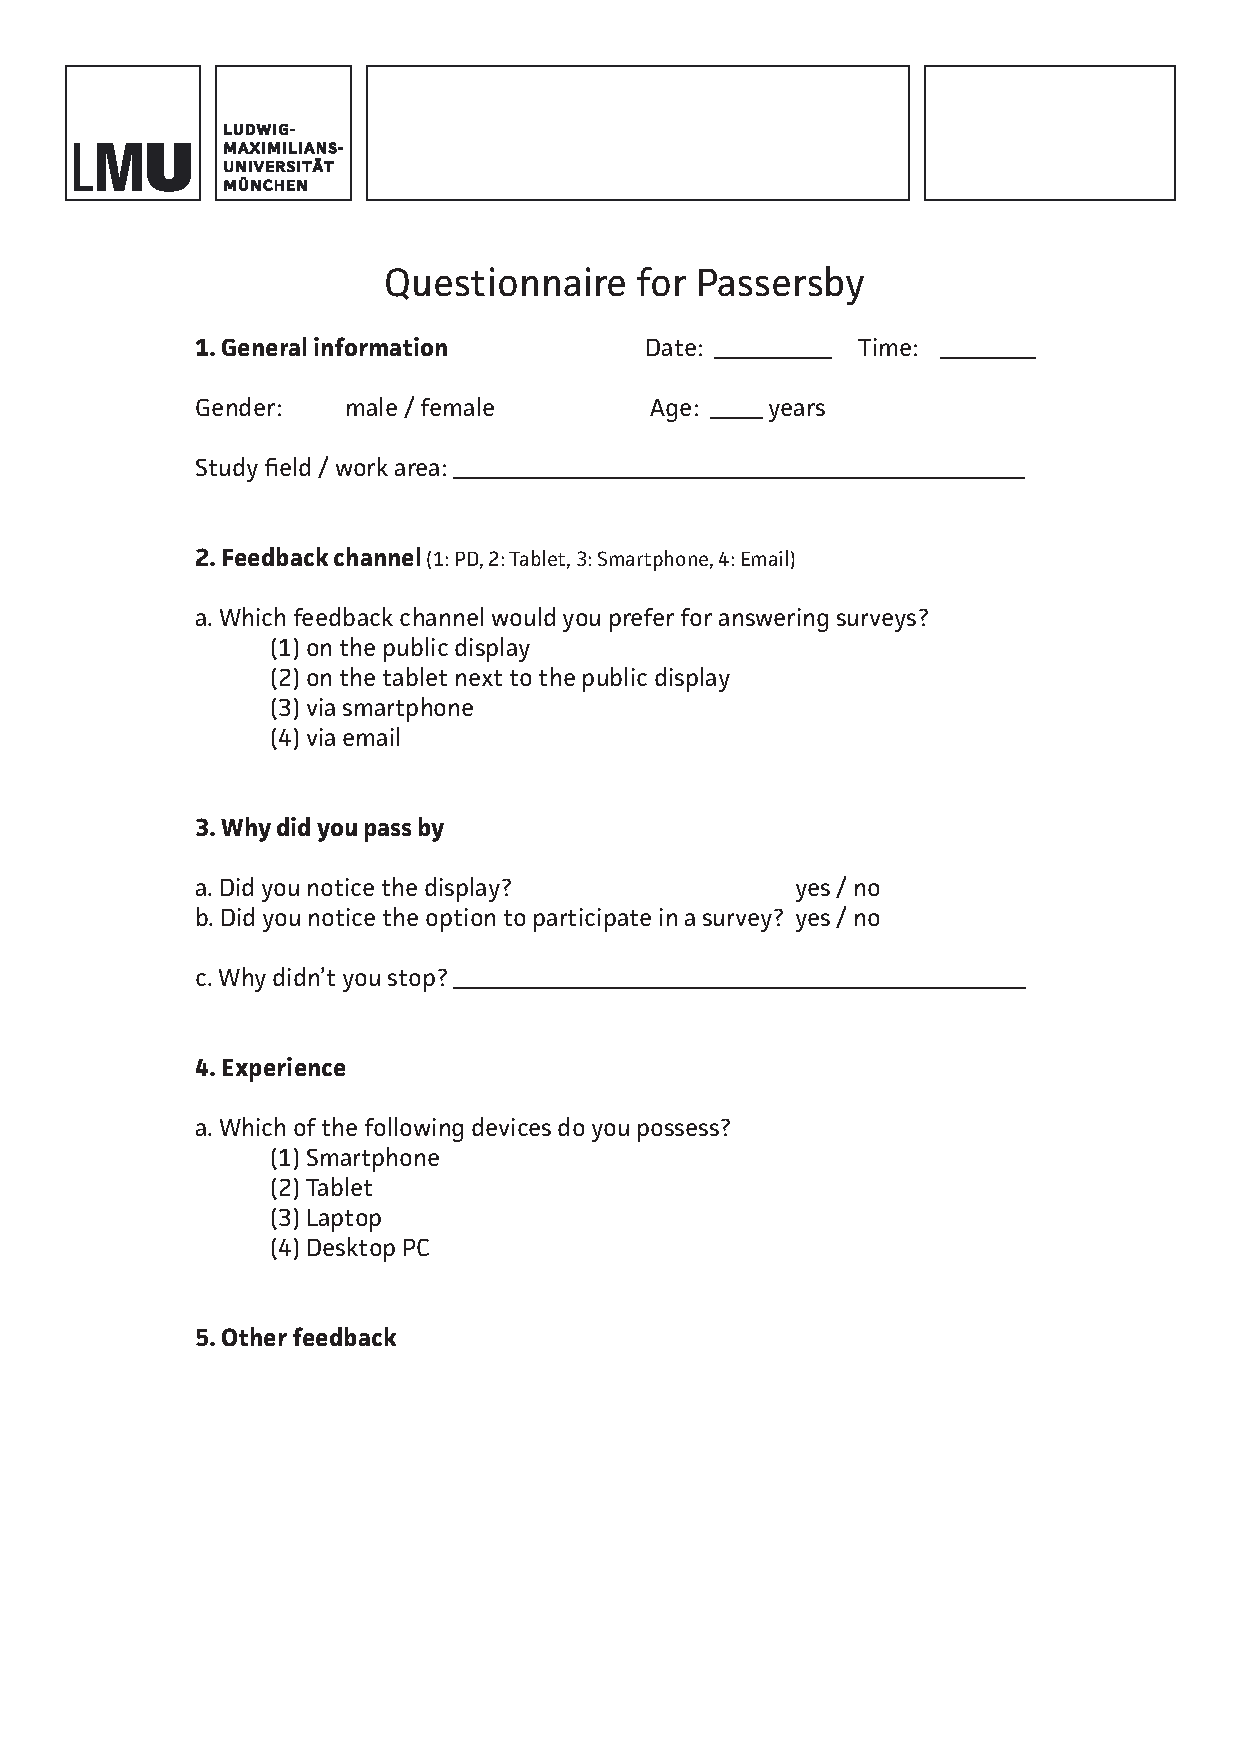
\includepdf[pages={-},scale=.9,pagecommand={}]{pdf/interview-passersby.pdf}

  \label{appendix:semi-structured-interview}
  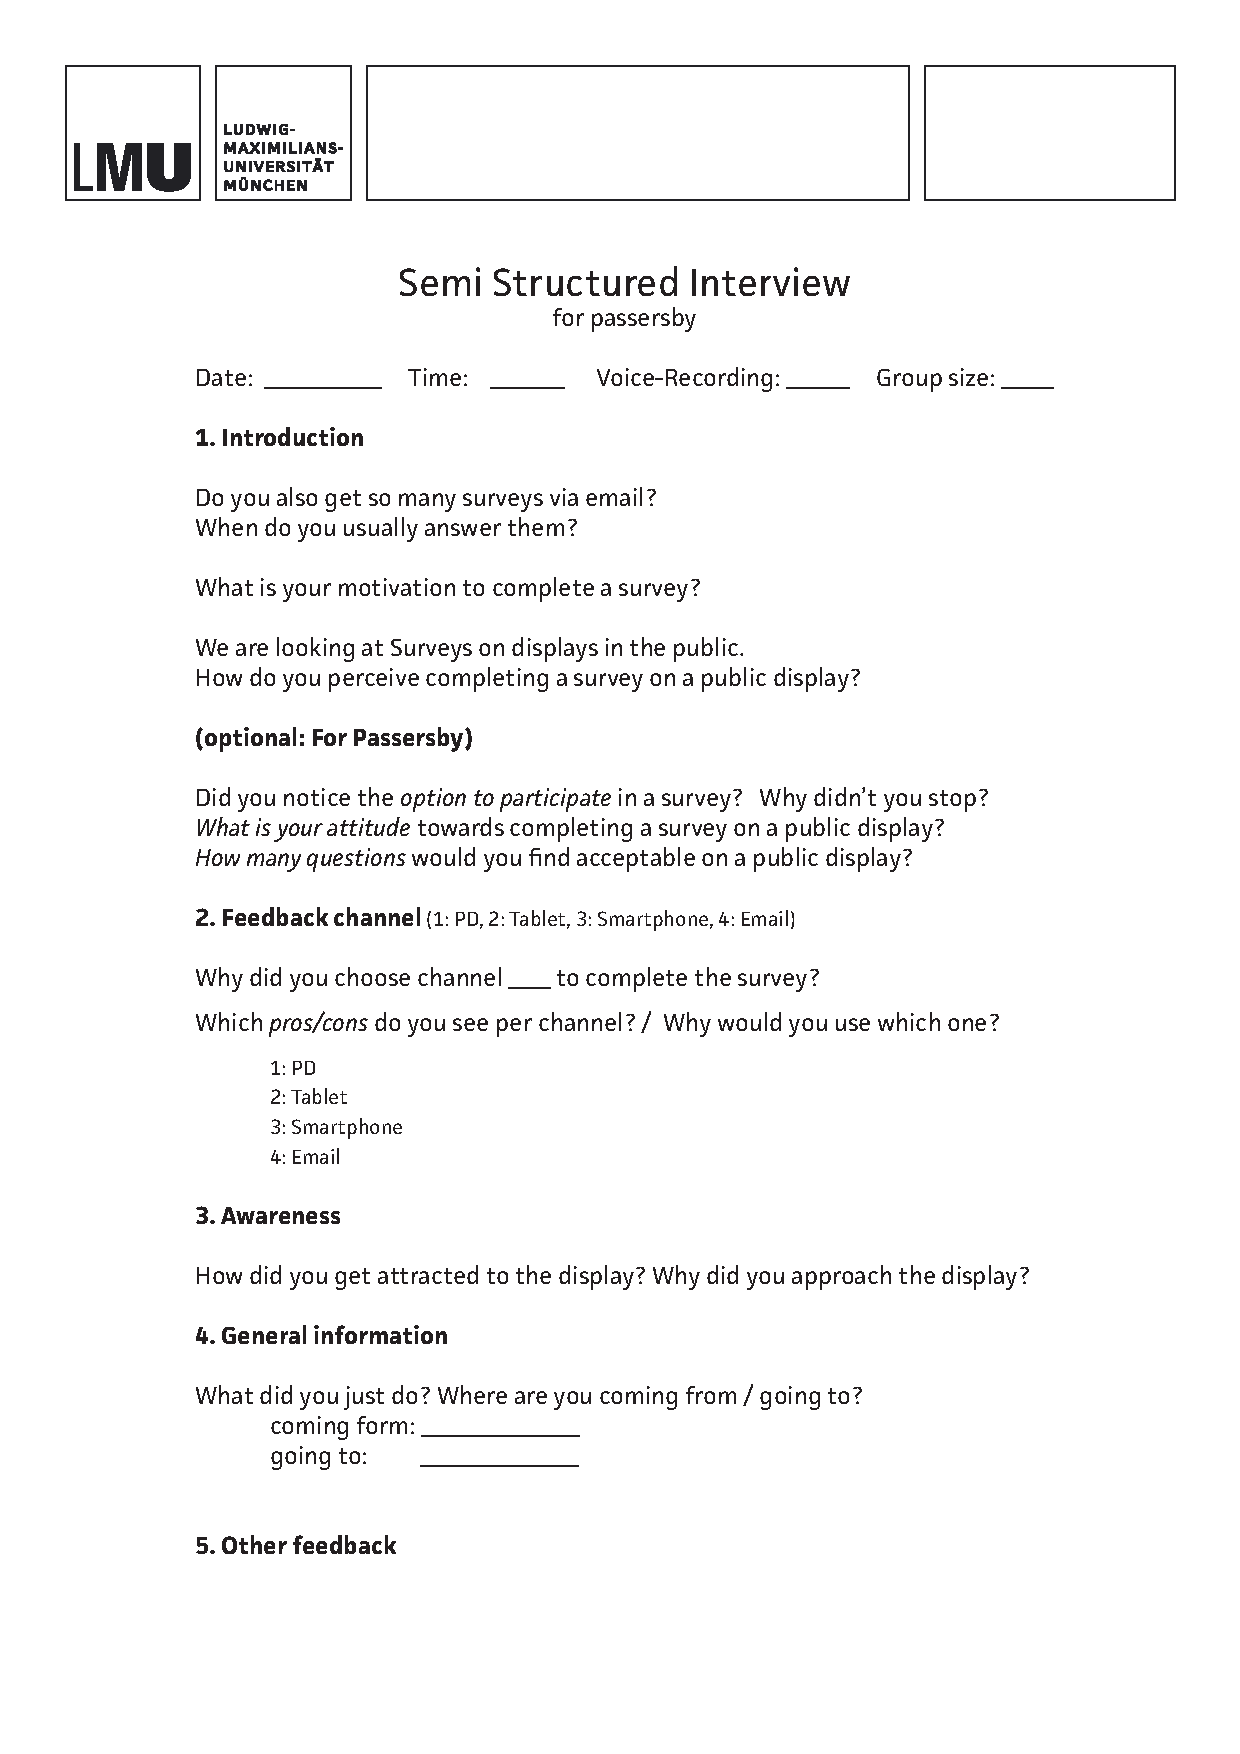
\includepdf[pages={-},scale=.9,pagecommand={}]{pdf/semi-structured-interview.pdf}



%% - - - - S C R E E N S H O T S - - - - %%
\clearpage
\section{Screenshots of Platform}
\label{appendix:screenshots-balloon-shooter}

    The following screenshots originate from the Balloon Shooter game developed by Jiamin Shi.


\paragraph{Options panel}
Each user saw this options panel after completing the Balloon Shooter game. Four channels were offered for completing the questionnaire. The order was randomized.
 \label{screenshot:options}
    \begin{center}
        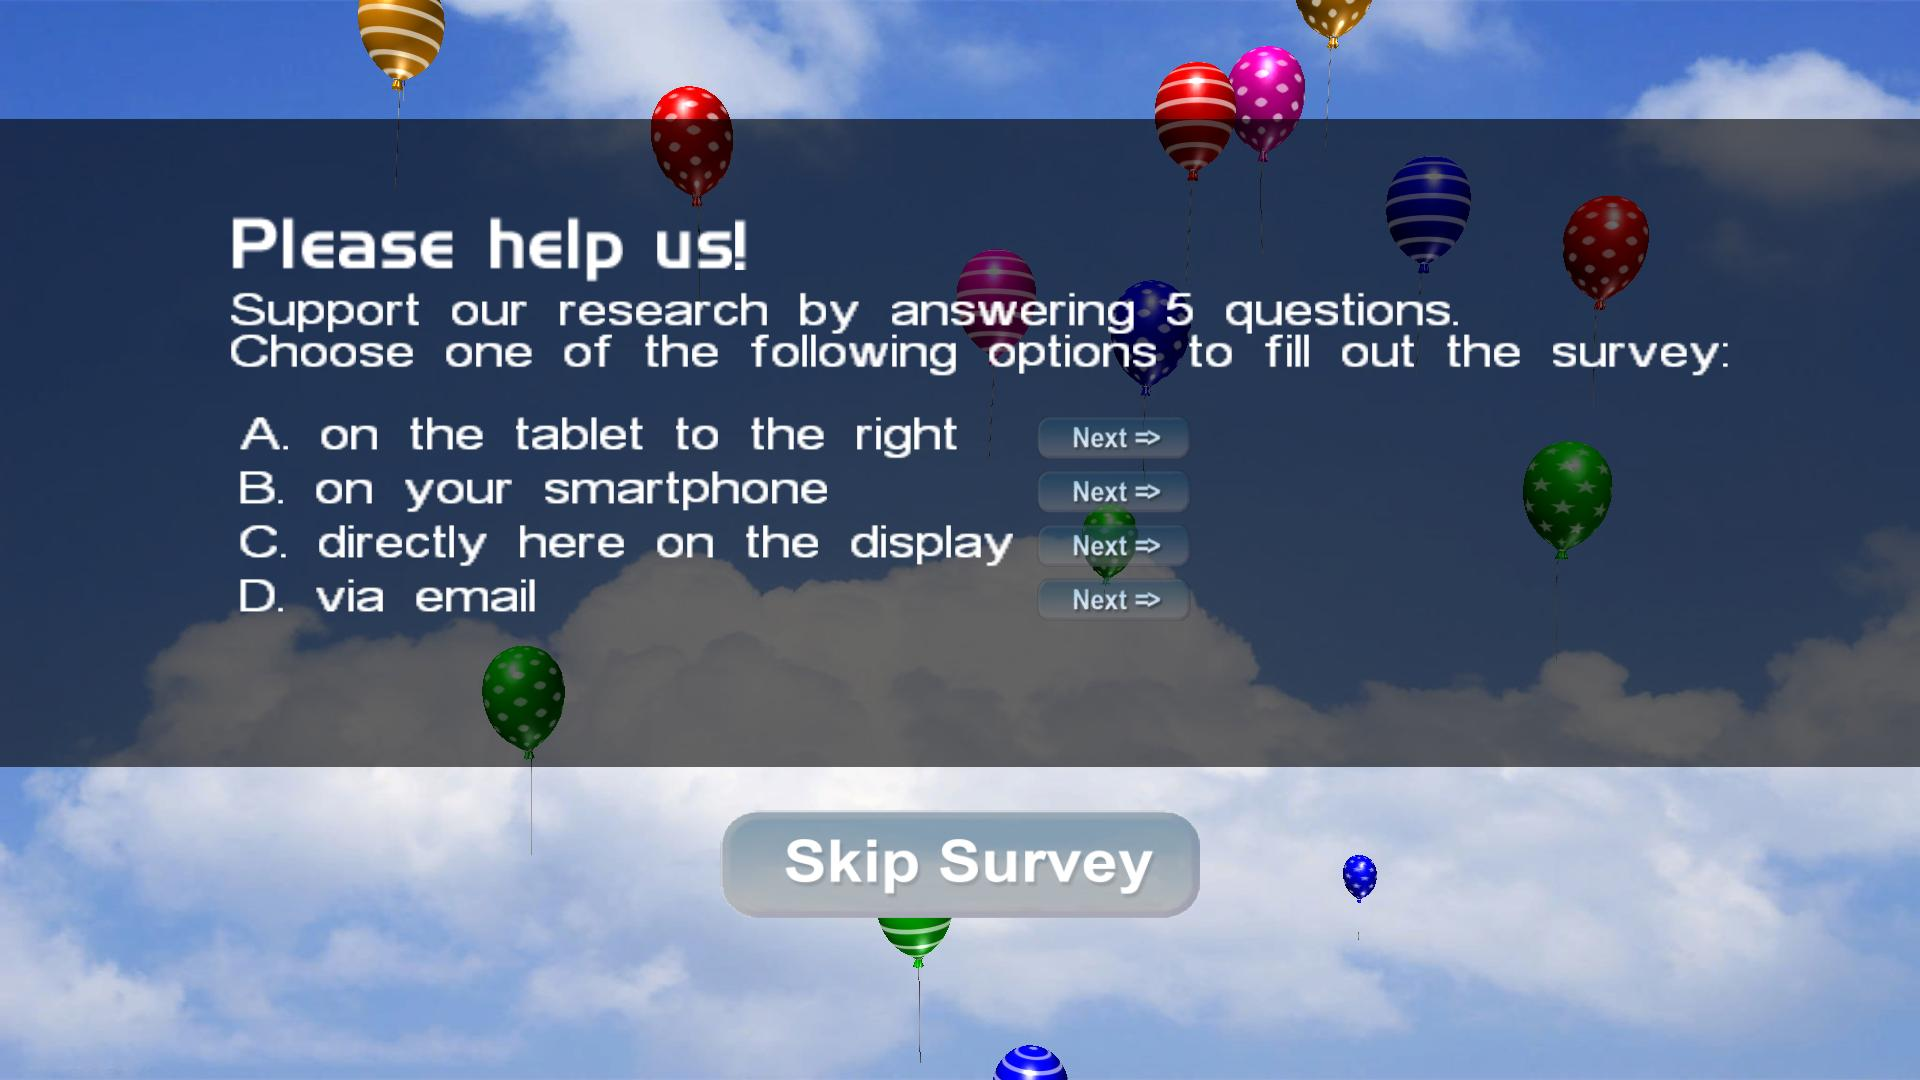
\includegraphics[width=\columnwidth]{img/screenshots/balloon-game/options-overview.jpg}
    \end{center}




\paragraph{Option: TV-Screen}
directly answering on the TV screen. Here you see a sample question getting asked on the interactive display.
 \label{screenshot:tv-option}

\begin{center}
    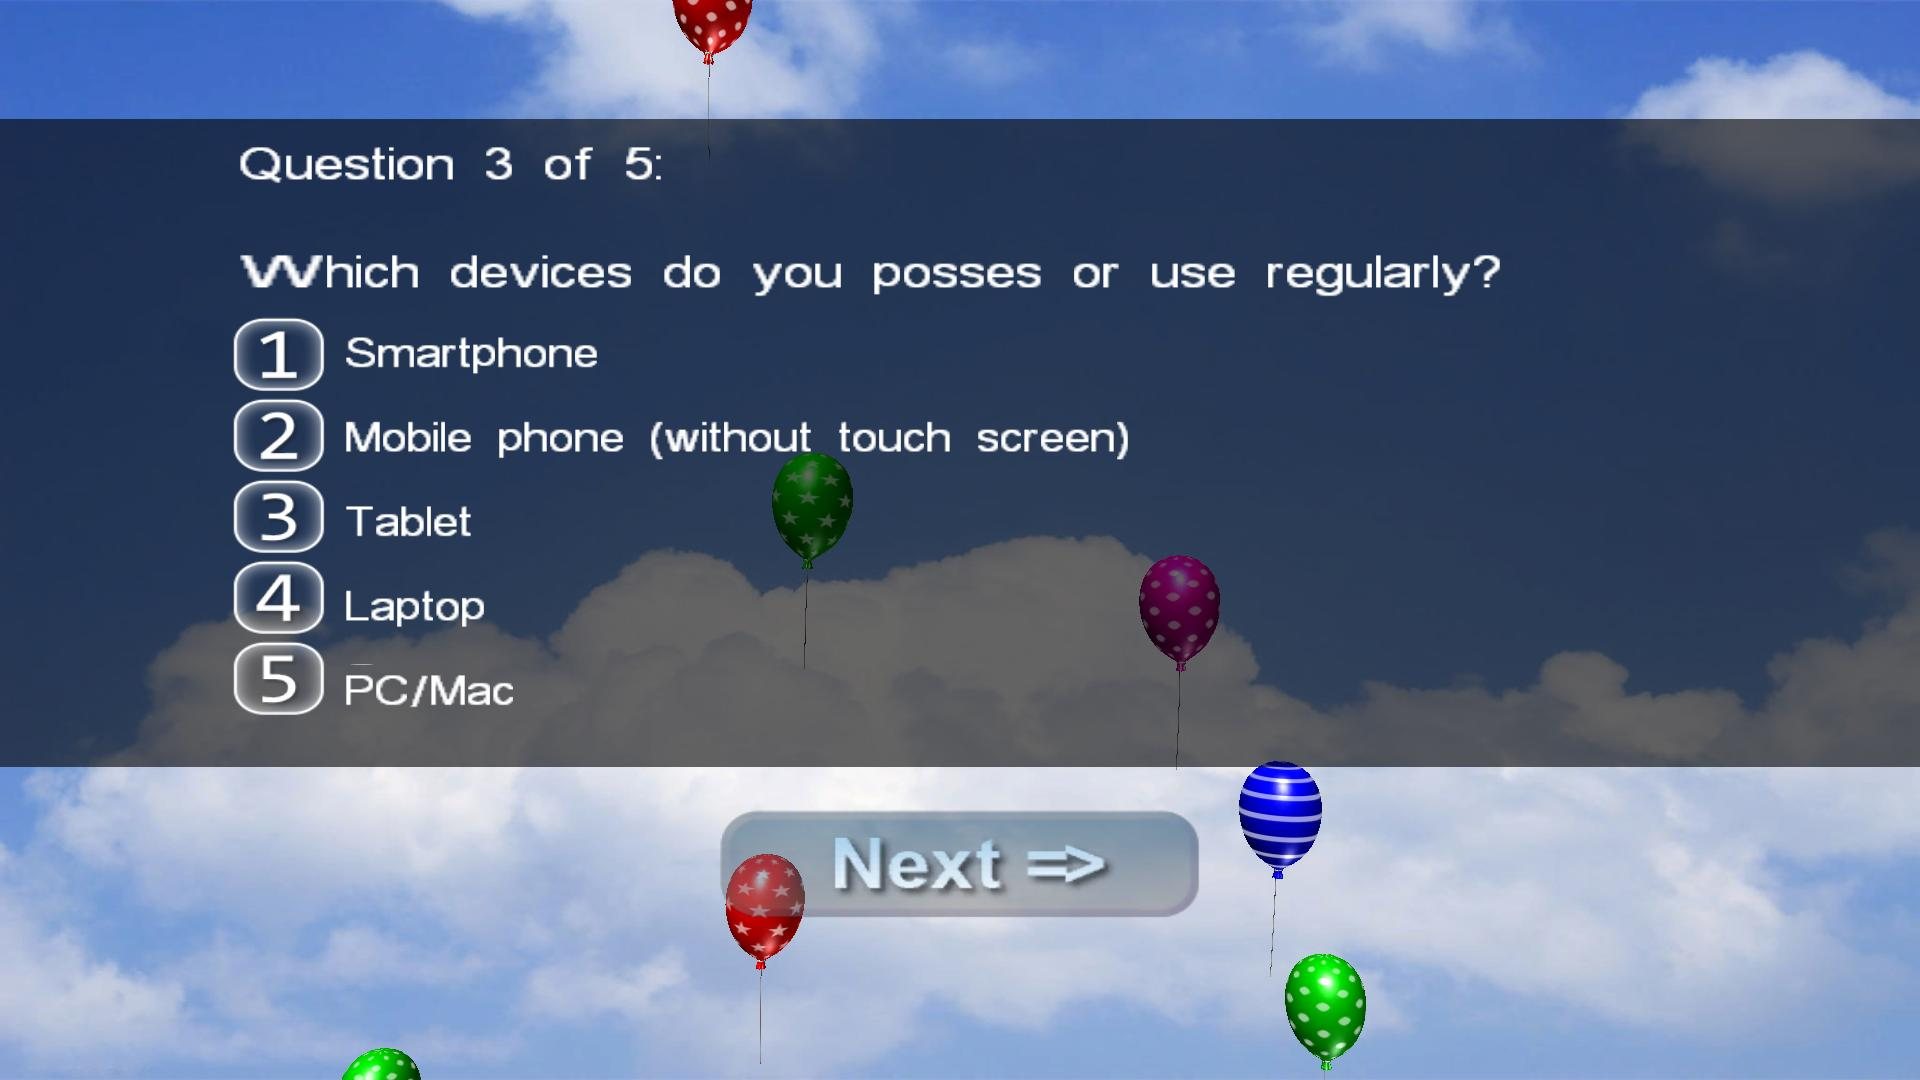
\includegraphics[width=\columnwidth]{img/screenshots/balloon-game/option-tv.jpg}
\end{center}




\clearpage

\paragraph{Option: Tablet}
\label{screenshot:tablet-option}
Option 2, the screen the user sees when choosing to complete the survey on the tablet

\begin{center}
    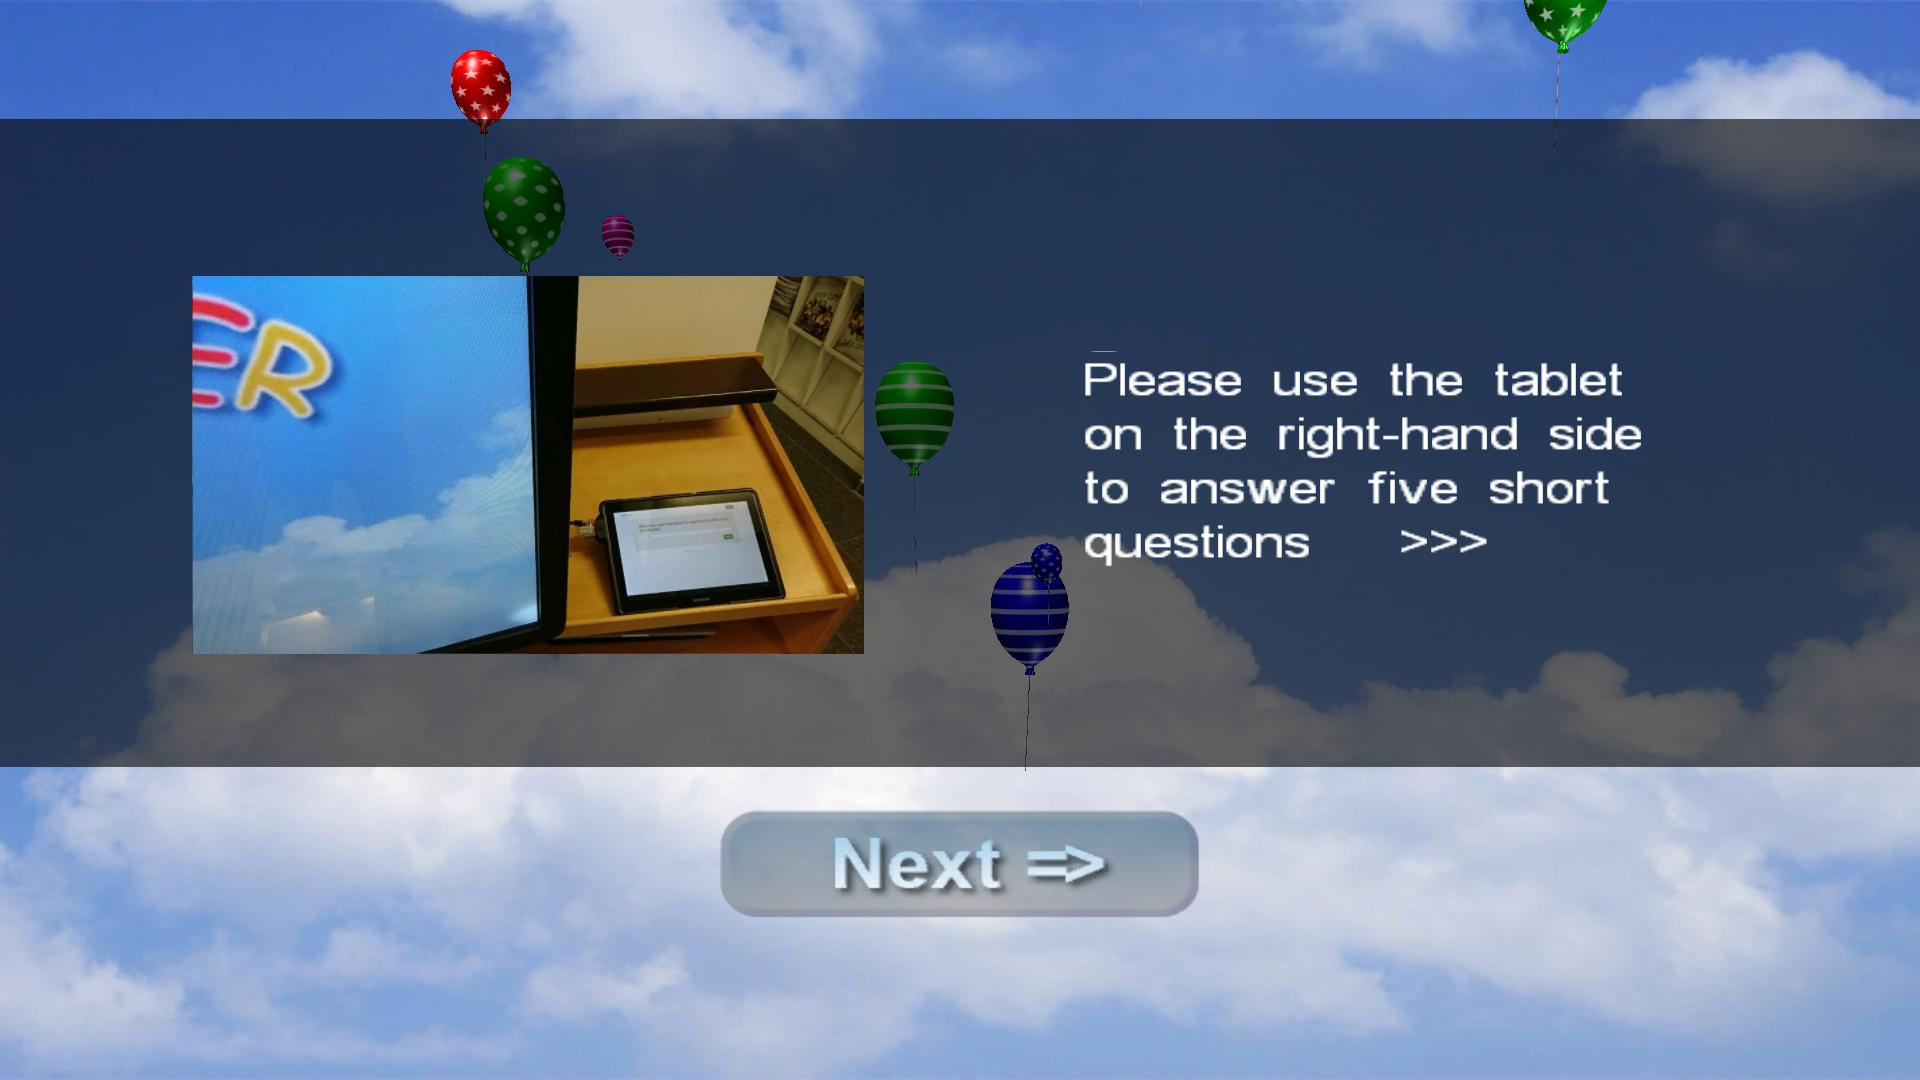
\includegraphics[width=\columnwidth]{img/screenshots/balloon-game/option-tablet.jpg}
\end{center}



\paragraph{Option: Smartphone}
\label{screenshot:smartphone-option}
Option 3, participating with your own smartphone, either by scanning the QR code or by typing the URL in the mobile browser

\begin{center}
    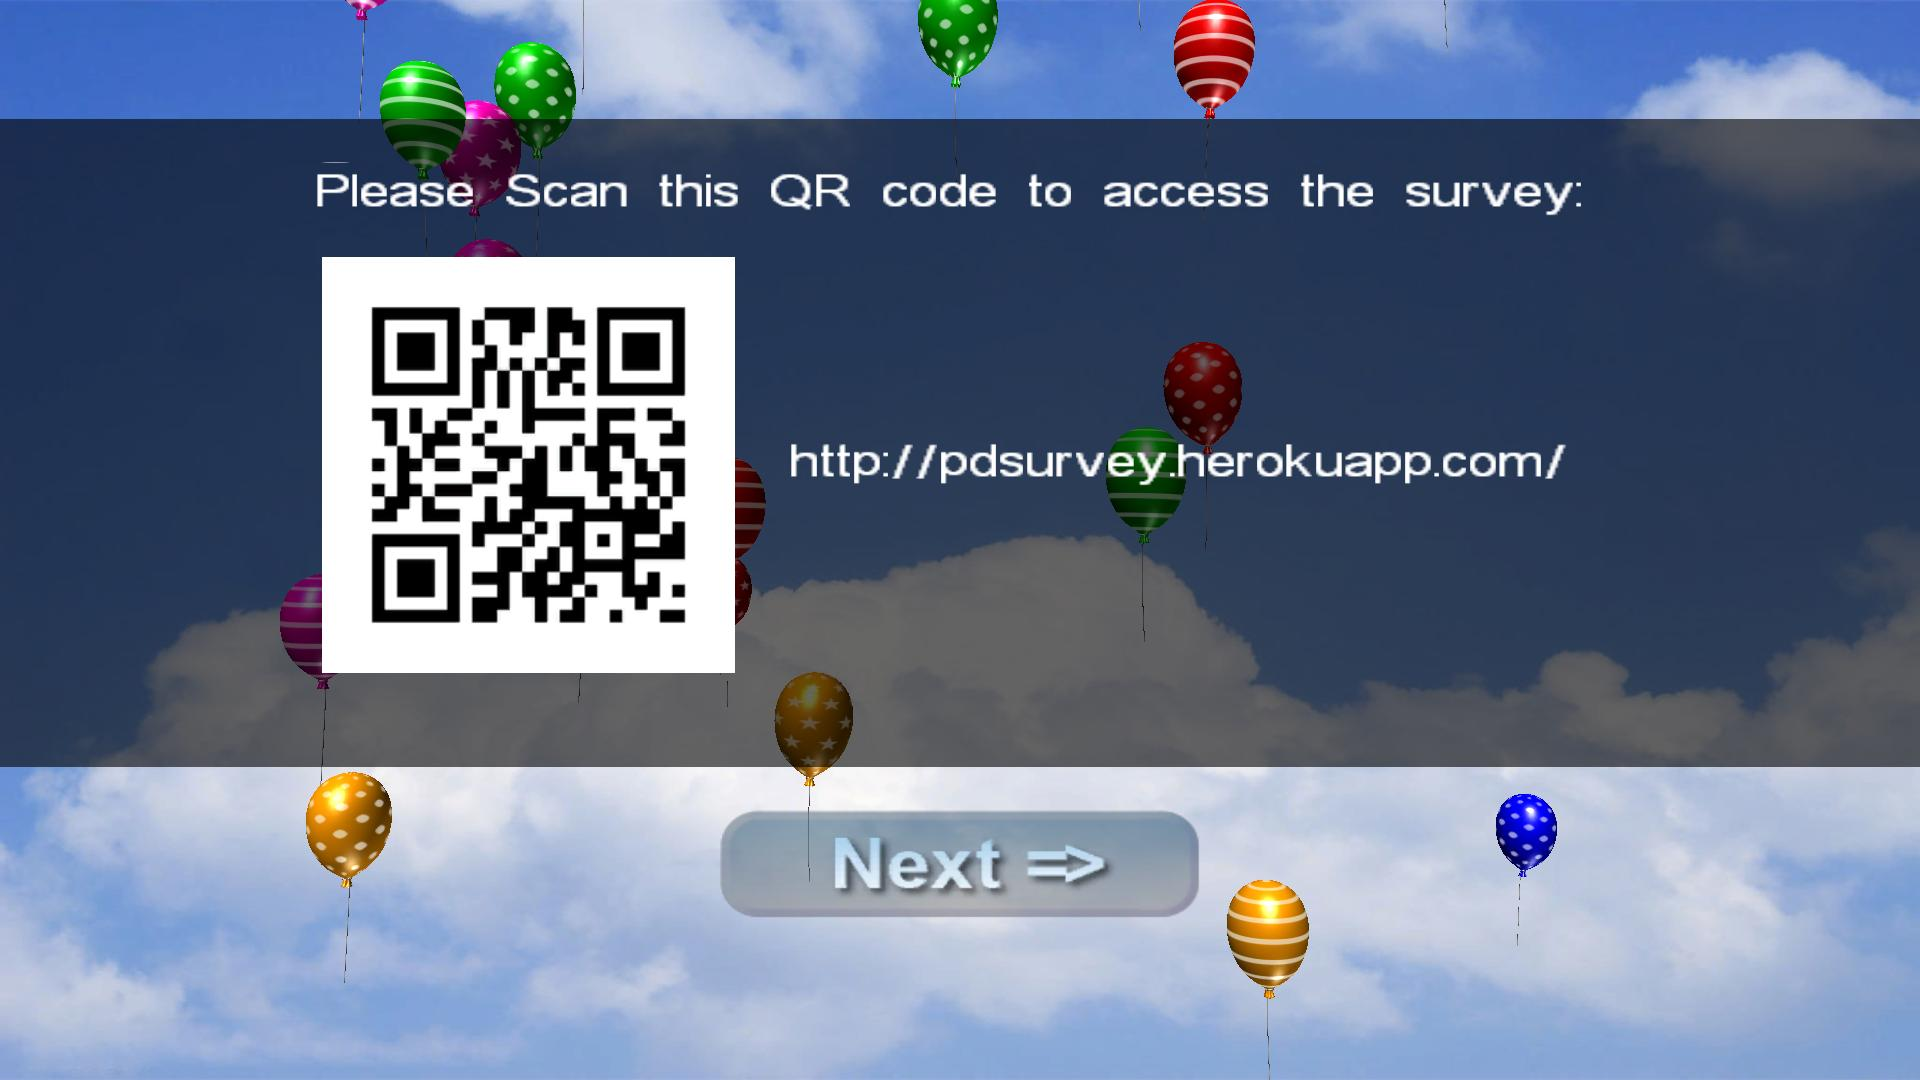
\includegraphics[width=\columnwidth]{img/screenshots/balloon-game/option-smartphone.jpg}
\end{center}




\clearpage
\paragraph{Option: Email}
\label{screenshot:email-option}
Option 4, submitting ones email address and getting the survey link to participate in response.

\begin{center}
    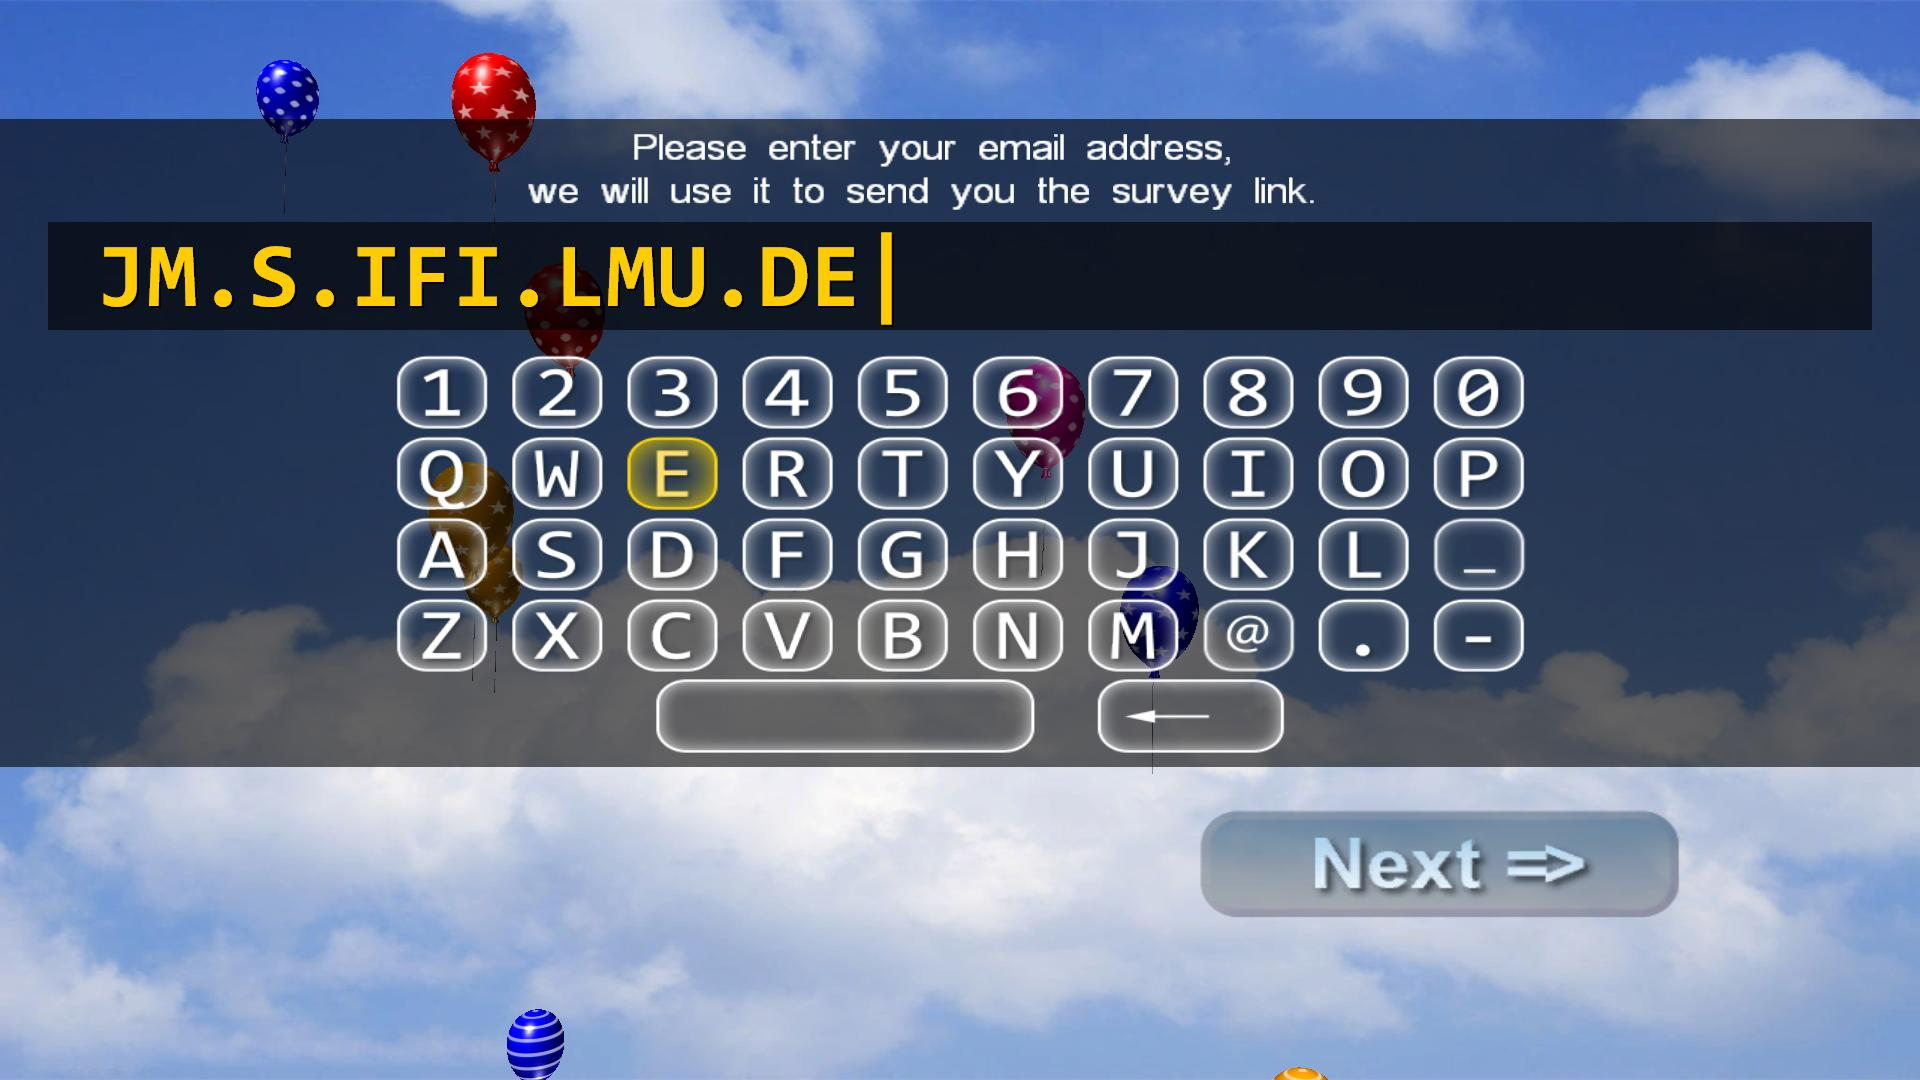
\includegraphics[width=\columnwidth]{img/screenshots/balloon-game/option-email.jpg}
\end{center}







%% LATEX HELP %%



% Table Notes

    % \begin{tablenotes}
          % \small
          % \item Sample description underneath the table. 
    % \end{tablenotes}